\documentclass[a4paper,11pt]{article}
\usepackage{amsmath,amsthm,amsfonts,amssymb,amscd,amstext,vmargin,graphics,graphicx,tabularx,multicol} 
\usepackage[francais]{babel}
\usepackage[utf8]{inputenc}  
\usepackage[T1]{fontenc} 
\usepackage{pstricks-add,tikz,tkz-tab,variations}
\usepackage[autolanguage,np]{numprint} 

\setmarginsrb{1.5cm}{0.5cm}{1cm}{0.5cm}{0cm}{0cm}{0cm}{0cm} %Gauche, haut, droite, haut
\newcounter{numexo}
\newcommand{\exo}[1]{\stepcounter{numexo}\noindent{\bf Exercice~\thenumexo} : \marginpar{\hfill /#1}}
\reversemarginpar


\newcounter{enumtabi}
\newcounter{enumtaba}
\newcommand{\q}{\stepcounter{enumtabi} \theenumtabi.  }
\newcommand{\qa}{\stepcounter{enumtaba} (\alph{enumtaba}) }
\newcommand{\initq}{\setcounter{enumtabi}{0}}
\newcommand{\initqa}{\setcounter{enumtaba}{0}}

\newcommand{\be}{\begin{enumerate}}
\newcommand{\ee}{\end{enumerate}}
\newcommand{\bi}{\begin{itemize}}
\newcommand{\ei}{\end{itemize}}
\newcommand{\bp}{\begin{pspicture*}}
\newcommand{\ep}{\end{pspicture*}}
\newcommand{\bt}{\begin{tabular}}
\newcommand{\et}{\end{tabular}}
\renewcommand{\tabularxcolumn}[1]{>{\centering}m{#1}} %(colonne m{} centrée, au lieu de p par défault) 
\newcommand{\tnl}{\tabularnewline}

\newcommand{\trait}{\noindent \rule{\linewidth}{0.2mm}}
\newcommand{\hs}[1]{\hspace{#1}}
\newcommand{\vs}[1]{\vspace{#1}}

\newcommand{\N}{\mathbb{N}}
\newcommand{\Z}{\mathbb{Z}}
\newcommand{\R}{\mathbb{R}}
\newcommand{\C}{\mathbb{C}}
\newcommand{\Dcal}{\mathcal{D}}
\newcommand{\Ccal}{\mathcal{C}}
\newcommand{\mc}{\mathcal}

\newcommand{\vect}[1]{\overrightarrow{#1}}
\newcommand{\ds}{\displaystyle}
\newcommand{\eq}{\quad \Leftrightarrow \quad}
\newcommand{\vecti}{\vec{\imath}}
\newcommand{\vectj}{\vec{\jmath}}
\newcommand{\Oij}{(O;\vec{\imath}, \vec{\jmath})}
\newcommand{\OIJ}{(O;I,J)}


\newcommand{\bmul}[1]{\begin{multicols}{#1}}
\newcommand{\emul}{\end{multicols}}

\newcommand{\reponse}[1][1]{%
\multido{}{#1}{\makebox[\linewidth]{\rule[0pt]{0pt}{20pt}\dotfill}
}}

\newcommand{\titre}[5] 
% #1: titre #2: haut gauche #3: bas gauche #4: haut droite #5: bas droite
{
\noindent #2 \hfill #4 \\
#3 \hfill #5

\vspace{-1.6cm}

\begin{center}\rule{6cm}{0.5mm}\end{center}
\vspace{0.2cm}
\begin{center}{\large{\textbf{#1}}}\end{center}
\begin{center}\rule{6cm}{0.5mm}\end{center}
}



\begin{document}
\pagestyle{empty}
\titre{Devoir maison : transformation du plan}{Nom :}{Prénom :}{Classe}{Date}

\bmul{2}

L'Alhambra situé en Andalousie (Espagne) est un complexe architectural islamique majeur considéré comme le plus majestueux du monde méditerranéen. En 1984, il a été déclaré site du patrimoine mondial.\\

Les mosaïques furent beaucoup utilisées dans la décoration de l'édifice et une des configurations les plus rencontrées est la "pajarita" (cocotte en papier). On la trouve par exemple sur la partie basse des murs du patio de los Arrayanes.\\



\columnbreak

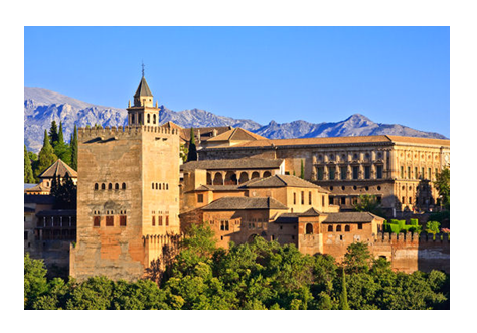
\includegraphics[scale=1]{alhambra.eps} 

\emul

Elle a servi à remplir l'espace délimité par des murs. On dit alors en langage mathématique que l'on a réalisé un pavage du plan à l'aide de ce motif.\\





\begin{center}
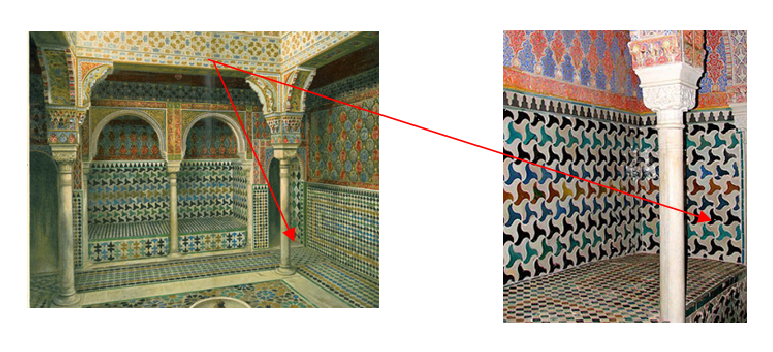
\includegraphics[scale=1]{alhambra2.eps} 
\end{center}




L'objectif de ce devoir est de réaliser un pavage à l'aide de ce motif que l'on va simplifier en utilisant le motif suivant toujours inspiré des pavages réalisés pour la décoration d'un des palais de l'Alhambra.\\

\textbf{A. Réalisation d'un motif}\\
\vspace*{0.3cm}


\underline{Programme de construction} :\\

\q Construire un triangle équilatéral ABC de cotés mesurant 8 cm.\\
\q Placer les points I milieu de [AB], J milieu de [BC] et K milieu de [AC].\\
\q Placer les points M milieu de [BJ], N milieu de [CJ], O milieu de [KC], P milieu de [AK], Q milieu de [AI] et R milieu de [IB].\\
\q	Tracer la droite perpendiculaire à (BC) passant par N et placer un point C1 sur cette droite à 1 cm de N à l'extérieur du triangle ABC.\\
\q	Tracer la droite perpendiculaire à (BC) passant par M et placer un point C2 sur cette droite à 1 cm de M à l'intérieur du triangle ABC.\\
\q	Tracer la droite perpendiculaire à (AC) passant par O et placer un point C3 sur cette droite à 1 cm de O à l'intérieur du triangle ABC.\\
\q	Tracer la droite perpendiculaire à (AC) passant par P et placer un point C4 sur cette droite à 1 cm de P à l'extérieur du triangle ABC.\\

\newpage
\vspace*{0.3cm}

\noindent \q	Tracer la droite perpendiculaire à (AB) passant par Q et placer un point C5 sur cette droite à 1 cm de Q à l'intérieur du triangle ABC.\\
\q Tracer la droite perpendiculaire à (AB) passant par R et placer un point C6 sur cette droite à 1 cm de R à l'extérieur du triangle ABC.\\



\bmul{2}
\noindent \q	Tracer l'arc de cercle de centre C1 passant par J.\\
\q	Tracer l'arc de cercle de centre C2 passant par J.\\
\q	Tracer l'arc de cercle de centre C5 passant par I.\\
\q	Tracer l'arc de cercle de centre C6 passant par I.\\
\q	Tracer l'arc de cercle de centre C3 passant par K.\\
\q Tracer l'arc de cercle de centre C4 passant par K.  \\


\columnbreak

\begin{center}
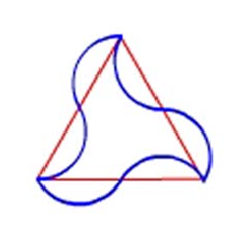
\includegraphics[scale=0.8]{alhambra3.eps} 
\end{center}
On obtient la figure ci-dessus.\\

\emul





\textbf{B. Réalisation du pavage}

\vspace*{0.3cm}

 A l'aide de transformations bien choisies, construire un pavage du plan à partir de la figure ci-dessus. Vous pouvez utiliser plusieurs transformations (la symétrie axiale, la symétrie centrale, la translation ou la rotation) pour obtenir votre pavage.\\
 Mettez ensuite de la couleur pour un meilleur rendu.\\
 


\begin{center}

\includegraphics[scale=0.8]{alhambra4.eps} 
\end{center}


\end{document}
